\documentclass[12pt]{article}
\usepackage{fullpage}
%\usepackage{fancyhdr}
\usepackage{color}
\usepackage{pdfpages}
\usepackage{hyperref}

\hypersetup{
	colorlinks=true,
	linkcolor=black,
	filecolor=magenta,      
	urlcolor=blue,
}

%\pagestyle{fancy}

\begin{document}
	\begin{titlepage}
	\begin{center}
		
	
	\vspace*{1in}
	{\Huge \textbf{FRC Advanced Control System Development: Part I}}\\
	\vspace{0.25in}
	{\LARGE CAN Diagnostic Stream \& CCSDSification}\\
	\vspace{0.5in}
	{\Large Carlos Gross Jones}\\
	\vspace{0.1in}
	{\Large FRC Team 696}\\
	\vspace{0.1in}
	{\Large \today}\\
\end{center}
	
\end{titlepage}


\section{Introduction}
\par This paper will cover a method of capturing CAN traffic on the RoboRIO, as well as encapsulating the CAN frames using the CCSDS Space Packet Protocol and transmitting them over the robot network. Later papers in this series will address how to capture, analyze, visualize, and log the resulting data streams. 


\section{Monitoring CAN Traffic}
\par Since so much of the communication on the robot occurs over the CAN bus (all PDP voltage/current telemetry, PCM status and commands, smart motor controller data, etc.), being able to monitor and process CAN frames immediately provides a wealth of telemetry and diagnostic information. A basic way of doing this is to simply use a device API to read the CAN data of interest, and then relay that data to a remote machine, using for example NetworkTables. However, this technique has several limitations. First, the telemetry is restricted to that data which can be accessed through existing API calls. Second, adding statements to poll effectively all APIs for all devices in use, and then publish that data, results in a tremendous amount of code cluttering up the user program. Futhermore, since a certain amount of decoding must be done by the RoboRIO, this would steal precious CPU cycles. 

\par Therefore, it is preferable to relay raw CAN frames to a remote machine, and process them on a more capable platform. There are several ways to do this. One would be to use some kind of CAN bridge physically connected to the bus, and to a data channel to the remote machine. The \href{https://copperhilltech.com/pican-2-can-interface-for-raspberry-pi-2-3/}{PiCAN2} and \href{https://www.microchip.com/DevelopmentTools/ProductDetails/PartNO/APGDT002}{Microchip CAN Bus Analyzer Tool} come to mind. However, since the RoboRIO already has a built-in CAN interface, as well as an Ethernet connection, it seems preferable to stream CAN frames from the RoboRIO, over Ethernet, across the WiFi link, to a telemetry computer. This allows realtime monitoring of all data that transits the CAN bus, in realtime, with minimal burden to the RoboRIO. 

\par First, a brief overview of the RoboRIO/Athena/WPIlib CAN stack is in order. The actual CAN interface on the RoboRIO PCBA is routed to the Zynq Z-7020 processor. The CAN interface to software is provided through FRCNetComm. User software then interacts with the FRCNetComm interface (either directly or via JNI). More specifically, CAN traffic is handled with the CANSessionMux framework. This allows multiple processes to send and receive packets through a single physical interface. \texttt{CANSessionMux.h} is reproduced in Appendix \ref{app:cansessionmux}.

\par Nearly all of the CAN communication commonly seen at the user level uses only the \texttt{sendMessage} and \texttt{receiveMessage} functions. The latter essentially monitors the incoming CAN traffic for a frame matching the ID parameter, and returns it when found. Unfortunately, this cannot be used to sniff CAN traffic, because \texttt{receiveMessage} ``steals'' frames; that is, if a process were set up to receive all frames, they would be consumed by that process and never reach the actual destination (robot code). However, the \texttt{*StreamSession} functions provide a much more flexible interface for inspecting CAN traffic. Essentially, user code merely sets up the stream session, optionally with an ID mask to exclude unneeded frames, and polls it occasionally. When polled, the stream returns all of the received CAN messages, \textit{without} affecting the normal reception of those frames in user code. Note that the \texttt{*StreamSession} functions are apparently so rarely used that they are not exposed in the CAN JNI. 

\section{CCSDS Encapsulation}
\par CCSDS, the Consultative Committee on Space Data Systems, maintains a Space Packet Protocol which is specifically designed for remote command and telemetry. The CCSDS header contains data to identify packet type, sequencing, and context. However, there are very few restrictions placed on the encapsulated data; the header is simply prepended to a block of data, from 1 to 65536 bytes. For these reasons, it is ideal for conveying robot telemetry to the remote machine. In order to pass the CCSDS packets over WiFi, they are simply sent as UDP datagrams. 



\newpage
\appendix

\section{CANSessionMux.h}
\label{app:cansessionmux}
\begin{verbatim}
#ifndef __CANSessionMux_h__
#define __CANSessionMux_h__

#include <stdint.h>

#define CAN_SEND_PERIOD_NO_REPEAT 0
#define CAN_SEND_PERIOD_STOP_REPEATING -1

/* Flags in the upper bits of the messageID */
#define CAN_IS_FRAME_REMOTE 0x80000000
#define CAN_IS_FRAME_11BIT  0x40000000

#define ERR_CANSessionMux_InvalidBuffer   -44086
#define ERR_CANSessionMux_MessageNotFound -44087
#define WARN_CANSessionMux_NoToken         44087
#define ERR_CANSessionMux_NotAllowed      -44088
#define ERR_CANSessionMux_NotInitialized  -44089
#define ERR_CANSessionMux_SessionOverrun   44050

struct tCANStreamMessage{
    uint32_t messageID;
    uint32_t timeStamp;
    uint8_t data[8];
    uint8_t dataSize;
};

#ifdef __cplusplus
namespace nCANSessionMux{
    void sendMessage_wrapper(uint32_t messageID, const uint8_t *data, 
                             uint8_t dataSize, int32_t periodMs, 
                             int32_t *status);
    void receiveMessage_wrapper(uint32_t *messageID, uint32_t messageIDMask, 
                                uint8_t *data, uint8_t *dataSize, 
                                uint32_t *timeStamp, int32_t *status);
    void openStreamSession(uint32_t *sessionHandle, uint32_t messageID, 
                           uint32_t messageIDMask, uint32_t maxMessages, 
                           int32_t *status);
    void closeStreamSession(uint32_t sessionHandle);
    
    
    
    
    void readStreamSession(uint32_t sessionHandle, 
                           struct tCANStreamMessage *messages, 
                           uint32_t messagesToRead, uint32_t *messagesRead, 
                           int32_t *status);
    void getCANStatus(float *percentBusUtilization, uint32_t *busOffCount, 
                      uint32_t *txFullCount, uint32_t *receiveErrorCount, 
                      uint32_t *transmitErrorCount, int32_t *status);
}
#endif

#ifdef __cplusplus
extern "C"{
#endif

    void FRC_NetworkCommunication_CANSessionMux_sendMessage(
            uint32_t messageID, const uint8_t *data, uint8_t dataSize, 
            int32_t periodMs, int32_t *status);
    void FRC_NetworkCommunication_CANSessionMux_receiveMessage(
            uint32_t *messageID, uint32_t messageIDMask, uint8_t *data, 
            uint8_t *dataSize, uint32_t *timeStamp, int32_t *status);
    void FRC_NetworkCommunication_CANSessionMux_openStreamSession(
            uint32_t *sessionHandle, uint32_t messageID, uint32_t messageIDMask, 
            uint32_t maxMessages, int32_t *status);
    void FRC_NetworkCommunication_CANSessionMux_closeStreamSession(
            uint32_t sessionHandle);
    void FRC_NetworkCommunication_CANSessionMux_readStreamSession(
            uint32_t sessionHandle, struct tCANStreamMessage *messages, 
            uint32_t messagesToRead, uint32_t *messagesRead, int32_t *status);
    void FRC_NetworkCommunication_CANSessionMux_getCANStatus(
            float *percentBusUtilization, uint32_t *busOffCount, 
            uint32_t *txFullCount, uint32_t *receiveErrorCount, 
            uint32_t *transmitErrorCount, int32_t *status);

#ifdef __cplusplus
}
#endif

#endif // __CANSessionMux_h__
\end{verbatim}
\newpage
\section{CCSDS Space Packet Protocol (Excerpt)}
\includepdf[pages=30-31]{CCSDS-SPP}

\end{document}
